
\section*{\textbf{\underline{Abstract}}}
The existence of patterns in population dynamics across species geographic ranges and climatic niches is a pervasive idea in ecology. Population variability (i.e., temporal variability in population density) should hypothetically increase near range edges or niche limits because of less suitable environments in these areas, but the occurrence of such patterns remains largely unexplored. Further, fluctuations in temperature could pose demographic constraints on populations and also influence their variability. We used the Breeding Bird Survey data to show that the population variability of 97 resident North American birds consistently increases towards their niche limits and in areas with more variable temperatures, but not towards their geographic range edges. However, our model has limited explanatory power, suggesting that other factors, such as biotic interactions and resource availability, might be more important drivers of population variability in resident North American birds.
%-----------------------
\section*{\textbf{\underline{Introduction}}}
%\section*{Introduction}
A general goal in ecology is to understand how species densities changes across geographic space and over time \parencite{lundberg2000,borregaard2010}. A commonly reported trend is that populations are more abundant the closer they are to the species geographic range center \parencite{brown1984, sexton2009}. Species climatic niches (i.e., the range of environmental conditions that allow species to persist indefinitely) are a main factor limiting species geographic distributions \parencite{pulliam2000, colwell2009}, such that these environmental conditions are assumed to be closer to the species optimum in the center of their geographic ranges, leading to higher density in these areas \parencite{brown1984,sagarin2006, pironon2017}. Despite being once regarded as a general rule \parencite{hengeveld1982}, evidence for the occurrence of geographic patterns in population density is limited \parencite{sagarin2002, sagarin2006, pironon2017, dallas2017}. This lack of support for these geographic trends could be occurring because geographic edges do not reflect climatic niche limits for many species \parencite{oldfather2019, pennington2021}, leading to the suggestion that population dynamics are more related to the position of populations within the species climatic niche \parencite{martinez2013,osorio2020}.  

\paragraph*{}
Perhaps a less explored consequence of patterns of population density across geographic and niche space is that population dynamics would be more variable the closer populations are to the edges of geographic ranges and climatic niches \parencite{lawton1993,sagarin2006, pironon2017}. As these populations would have lower densities, demographic stochasticity becomes an important driver of their dynamics, leading populations to be more variable near range edges or niche limits \parencite{melbourne2008, pironon2017, tencaten2025}. Understanding how populations vary across species geographic ranges and climatic niches is of particular importance given that increasing fluctuations in population densities are associated with higher extinction risk \parencite{bjornstad2001, ovaskainen2010}, and the detection of such trends could inform conservation efforts \parencite{burgess2020}. However, differences in how population variability is structured across geographic ranges or climatic niches have rarely been assessed \parencite{sagarin2006,pironon2017, tencaten2025} despite being considered prevalent across species \parencite{vucetich2003}.
 
\paragraph*{}
Different extrinsic (environmental) and intrinsic (demographic) factors may affect population variability irrespective of population position within the species climatic niche or geographic range. For example, increased fluctuations in environmental conditions lead to more variable population dynamics given that extreme environments are more likely to pose demographic constraints on populations \parencite{bjornstad2001, boyce2006}. Species traits, such as body size and dispersal ability, may also influence patterns of population variability across geographic and climatic space. For instance, fluctuations in population densities are often associated with changes in body sizes \parencite{chitty1952,van2017} while dispersal usually stabilizes population dynamics \parencite{doebeli1995,abbott2011}. Several of these traits that affect population dynamics are phylogenetically conserved \parencite{wiens2010, park2015}, indicating that there could be a phylogenetic signal in patterns of population variability \parencite{dallas2024}.
 
\paragraph*{}
The influence of geographic ranges and climatic niches on population variability represents a major knowledge gap in our understanding of population dynamics. Differences in environmental conditions that populations experience are considered important drivers of patterns of population dynamics across geographic ranges and climatic niches \parencite{sagarin2006,pironon2017, tencaten2025}, but the effects of environmental factors are often ignored during the assessment of these relationships. Here we address these gaps and examine the effects of climatic niche position, geographic range position, and temperature variability on the population variability of 97 resident North American bird species (Figure \ref{fig:concep_varrange}). Phylogenetic history and species differences in body size and dispersal ability were considered to assess their influence on these relationships. We hypothesized that population variability would be more strongly related to climatic niche position and temperature variability than geographic range position. We expected this given that niches impose boundaries to the climatic conditions where populations can have positive growth rates and because temperature fluctuations can move populations along the species niche, and in some cases even beyond niche limits, influencing their variability. Alternatively, geographic range edges might not represent niche limits (Figure \ref{fig:rangelimits}) and can have suitable environmental conditions that could buffer population variability \parencite{oldfather2018}. We also expected that closely related species were going to exhibit similar patterns of population variability, and that species body size and dispersal ability would influence these relationships.  
 
%-----------------------
\section*{\textbf{\underline{Methods}}}
%\section*{Methods}
\paragraph*{Estimating population variability}\mbox{}\\ 
We used the North American Breeding Bird Survey (BBS; \textcite{sauer2020}) data to estimate yearly densities of 99 resident bird species. Species sampled by BBS were classified as resident based on \textcite{rosenberg2019}. The BBS is an annual standardized census of North American breeding birds. The surveys are conducted by skilled volunteers during the breeding season where survey routes of $\approx$ 50km are sampled every 1km (i.e., a total of 50 stops) for about 3 minutes through point counts where all birds seen or heard within a 0.4km radius are recorded. We only considered resident species because migratory birds might be exposed to different environmental conditions in their breeding and non-breeding ranges \parencite{ponti2020} that could affect their survival. Many migratory birds also have a substantial portion of their geographic ranges in areas outside of North America that are not sampled by BBS. Resident species could still have only a small portion of their geographic ranges sampled by BBS, but restricting our analysis to consider only resident species that had $\geq$70\% of their geographic ranges sampled by BBS yielded the same results as when considering all resident species (see Appendix C for details). BBS data was obtained through the \texttt{bbsAssistant} R package \parencite{burnett2019}.


We used the data sampled between 1997 and 2019 to estimate population variability for the  species considered in our study. The species considered in our study have been recorded in a total of 4803 routes since 1997. Each route has been sampled on average for 15$\pm$7 years and an average of 3051$\pm$127 routes were surveyed by BBS yearly between 1997 and 2019 (Figure \ref{fig:routes}). Population variability was estimated as the coefficient of variation (hereafter CV; $CV = \frac{\sigma}{\mu}$), relating the standard deviation in temporal dynamics of a population ($\sigma$) to it's mean ($\mu$) in density in a site. Only sites where species were recorded for at least five different time periods (mean of 371$\pm$600 sites) were considered in our calculations. Population variability was estimated considering only the years a species was observed to occur in a target site. We also explored whether a more conservative estimate of population variability, only considering sites where species were observed to occur in at least 10 years, influenced the observed relationships. Alternatively, we also considered a less conservative estimate of population variability, where we assigned a density of zero to sampling events where a species was not recorded in a site, but that sampling event was done between the first and last year that a species was recorded at a given site to investigate whether this assumption affects our results. %In this case, it is possible for a species that was observed five times in a site to have density of zero for three years and density > zero for the two other years. 

\paragraph*{Estimating geographic ranges, realized climatic niches, and temperature variability}\mbox{}\\ 
We estimated species geographic ranges as minimum convex polygons considering all BBS sampled points. The minimum convex polygon is defined as the smallest area that connects all sampled points that a species was recorded at with no interior edge. We opted to build our own polygons rather than using expert-derived ranges because of potential problems associated with using expert ranges. For example, expert estimates of a species geographic range can be disjunct, which can lead to the center of the range falling outside the species geographic range and there might also be observations that fall outside of expert ranges  \parencite{fristoe2023}, which could affect the assessment of these relationships. The center of the species geographic range was defined as the centroid of the species ranges. Geographic range centers were also estimated using expert ranges obtained from birdLife \parencite{birdlife} rather than minimum convex polygons and we also used distance to range edge as an alternative measure of geographic range position and found similar results (see Appendix C). 


To estimate the realized climatic niche of the species in our study, we used the 19 bioclimatic variables, consisting of quantities related to temperature and precipitation relevant to species life history (e.g., temperature seasonality, temperature of coldest month, etc.), available in the CHELSA database \parencite{karger2017}. These variables are considered main drivers of North American birds distribution and abundance \parencite{barbet2014, illan2014, huang2017}. Bioclimatic variables were obtained at a resolution of 0.008$^\circ$, and were aggregated to 0.5$^\circ$. to match the resolution of sampled BBS sites. We performed a principal component analysis (PCA) over these variables, and used the first two axes (explained $\approx$ 80\% of the variance in the data) to estimate realized climatic niches. We extracted environmental values from these two PCA axes and used minimum convex polygons to determine species realized climatic niches (see Figure \ref{fig:concep_varrange}). The centroid of these polygons were used to represent the center of climatic species niches. Climatic niches were also estimated using expert ranges and we observed similar results (see Appendix C for details).  

To estimate temperature variability, we obtained monthly mean temperature data for the years of 1997-2019 also from CHELSA database at a resolution of 0.008$^\circ$. that were aggregated to 0.5$^\circ$. To account for the different number of cells potentially being aggregated across different latitudes due to conformal projection, we also reprojected and aggregated mean monthly temperature data using Behrmann equal area projection (see details in Appendix C). We estimated the coefficient of variation in temperature for each year and site where species were sampled to use as an estimate of temperature variability that populations experienced. 
\paragraph*{The relationship between population variability and geographic ranges, climatic niches, and temperature fluctuations}\mbox{}\\ 
To evaluate how population variability was related to geographic range position, niche position, and temperature variability we fit linear mixed models. Two species (\textit{Strix nebulosa} and \textit{Megascops kennicottii}) that were sampled in fewer than five sites for at least five years were removed from our analyses. Population variability was the response variable and geographic range position, climatic niche position, and mean annual temperature variability were fixed effects in these models. Species were used as random effects (considering a reduced-rank covariance structure) to estimate the slope of the relationship between population variability and the fixed effects for each species separately. Thus, our models had random slopes, but not random intercepts, as random effects. All variables were standardized to have a mean of zero and a standard deviation of one prior to fitting the models. Linear mixed models were fit using a Gaussian family with the \texttt{glmmTMB} R package \parencite{brooks2017} and we performed model diagnostics (see Figure \ref{fig:main_mod} and Appendix C for details) and estimated model goodness of fit (Nakagawa's conditional $R^2$) using the \texttt{performance} R package \parencite{ludecke2021}. This conditional $R^2$ takes fixed and random effects into account when estimating the model goodness of fit.
\paragraph*{Assessing the effects of phylogeny and species traits on patterns of population variability}\mbox{}\\ 
Information on body size and dispersal ability for each species was obtained from the AVONET database \parencite{tobias2022}. We used body mass as a measure of body size and the hand-wing index as a measure of dispersal ability. Measuring the dispersal ability of birds is a challenging task, and for that reason biometric indices have often been used to describe their dispersal ability \parencite{sheard2020}. The hand-wing index considers information on flight efficiency and metabolic demands \parencite{claramunt2012,claramunt2017} and is positively related to the dispersal ability of birds \parencite{arango2022}. We used the crosswalk taxonomy from AVONET \parencite{tobias2022} to link the taxonomies from BirdLife and BirdTree \parencite{jetz2012bird} to obtain phylogenetic information for the 97 resident species considered in our analyses. We removed \textit{Aphelocoma woodhouseii} from our phylogenetic analyses because its equivalent species in BirdTree was a duplicate in our dataset (i.e., it was already present in our dataset). Thus, the phylogeny we used to assess whether species traits affect trends in population variability had 96 species.

We extracted the random slopes for each species from our linear mixed model and estimated Pagel's $\lambda$ and Blomberg's $K$ to assess whether there is a phylogenetic signal in how population variability is structured as a function geographic range position, climatic niche position, and temperature variability across species. Phylogenetic signal was estimated using the \texttt{phytools} package \parencite{revell2012}. We also fit three phylogenetic generalized least squares (PGLS) to explore how the species slopes changed as a function of log-transformed body size and log-transformed dispersal ability. PGLS models were fit using the \texttt{caper} R package \parencite{caper}.

%-----------------------
\section*{\textbf{\underline{Results}}}
%\section*{Results}
\paragraph*{Is population variability related to geographic range position, climatic niche position, or temperature variability?}\mbox{}\\ 
We found that the population variability of resident North American birds increases near climatic niche limits and in areas that have more variable temperature (Table \ref{tab:lmm_main}). These results were consistent regardless of how population variability, climatic niches, and temperature variability were estimated (see Appendix C). The relationship between population variability and geographic range position was inconsistent and depended on how population variability was estimated, but not on how geographic ranges or range position were estimated (Tables \ref{tab:lmm_exp}-\ref{tab:lmm_edge} ). There was no relationship between population variability and geographic range position when population variability was estimated considering cases where species were observed at least five years in a site. However, these relationships became significant when zeros were considered when estimating population variability or when we only used populations that occurred in sites for at least 10 years (Tables \ref{tab:lmm_zeros}-\ref{tab:lmm_tens}). Nevertheless, conditional $R^2$ in our models were often $\approx$ 0.01, suggesting that most of the variance in these relationships remained unexplained. 

\paragraph*{Do phylogenetic history and traits affect population variability responses across species?}\mbox{}\\ 
There was no phylogenetic signal in the effects of climatic niche position ($\lambda  < 0.01, p = 1; K = 0.02, p = 0.81$) or temperature variability ($\lambda < 0.01, p = 1; K = 0.01, p = 0.92$) on population variability across species. There was some evidence for phylogenetic signal ($\lambda  < 0.01, p = 1; K = 0.10, p = 0.04$) in how population variability was related to geographic range position (Figure \ref{fig:phylo}). Species with smaller body sizes had less variable populations near geographic range edges, but not near niche limits or in variable temperatures while dispersal ability was unrelated to patterns of population variability. These models were unable to explain most of the variance in patterns of population variability across species ($R^2 \approx$ 0.1, Table \ref{tab:PGLS}). 
%-----------------------
\section*{\textbf{\underline{Discussion}}}
%\section*{Discussion}
Population variability is predicted to increase in areas that have unsuitable environmental conditions such as near geographic range edges and climatic niche limits or in climatically variable locations  \parencite{pironon2017,burgess2020,tencaten2025}, but there are limited empirical assessments of these expectations. We found that the population variability of resident North American birds consistently increases near climatic niche limits and in areas that have more variable temperatures, but not near geographic range edges. However, our models could not explain most of the variation in these relationships, and phylogenetic history and traits did not influence species differences in population variability. The limited explanatory power of these relationships may be because several factors, such as resource availability and biotic interactions, can simultaneously influence population variability \parencite{lundberg2000, tencaten2025}, which could obscure these patterns across geographic and niche space or in variable temperatures. The suitability of environmental conditions across geographic and niche space might also not exhibit a homogeneous gradient of more to less suitable conditions from center towards the edges of ranges or niches as previously suggested \parencite{brown1984, martinez2013}. This would lead to noisier relationships between population variability and their position within geographic and climatic niche space of species.  
  
\paragraph*{}
Increased population variability near climatic niche limits and in variable temperatures is possibly due to the harsh boundaries that niche limits impose on populations \parencite{sexton2009,hargreaves2014} and because temperature variability causes fluctuations in population growth rates and lead to more variable dynamics \parencite{lande1993}. Geographic range edges may represent physical barriers, such as mountains and terrestrial boundaries, and not niche limits for several species and can have suitable environmental conditions that might buffer population variability in these areas \parencite{oldfather2018,oldfather2019, pennington2021}. However, assigning a density of zero to sampling events where species were not recorded in sites or considering only sites that were sampled for over 10 year led to higher population variability near range edges. This suggests that sites that are only occupied temporarily by species influence observed patterns of population variability and that time series length might also be important to detect these relationships (\parencite{pimm1988}; see Appendix C for details). Nonetheless, individual populations can exhibit adaptations to local environmental conditions, and have different climatic niche limits, that could mitigate their variability \parencite{demarche2018,oldfather2019}. Such local adaptations, coupled with the occurrence of demographic compensation (i.e., opposing vital rate trends in different environments \parencite{doak2010,villellas2015}), might weaken the influence of climatic niche position, geographic range position and temperature variability on population variability.

\paragraph*{}
Species that have smaller body sizes often exhibit higher fluctuations in population density than larger-bodied species \parencite{lawton1994}, but we did not observe a consistent effect of body size on patterns of population variability. The inability of body size to explain species differences in patterns of population variability can be due to other factors (e.g., level of ecological specialization and habitat loss) possibly regulating the effects of body size on population dynamics \parencite{owens2000,cowlishaw2009}. Although dispersal of individuals influence population dynamics \parencite{doebeli1995, abbott2011}, species dispersal ability was unrelated to population variability patterns. Experimental evidence shows that, in many scenarios, dispersal does not affect population variability \parencite{yang2022}, indicating that dispersal ability may be unable to explain species differences in patterns of population variability. The lack of phylogenetic signal in these relationships also suggests that the factors that influence patterns of population variability are highly variable across North American bird species.

\paragraph*{}

The extent to which these findings are generalizable to other taxa is an interesting open question as the effects of geographic range position, climatic niche position, and temperature fluctuations on population variability may depend on life history traits. Considering the influence of species level properties on the strength of these relationships may also further our understanding of these macroecological patterns. For instance, do species with larger geographic ranges also tend to have more variable populations near range edges? How does climatic niche breadth influence these relationships? By leveraging population dynamic theory \parencite{roughgarden1975,levin1976}, along with ideas from physiological ecology about species performance curves \parencite{buckley2008,tencaten2025}, it may be possible to generate testable predictions from theory about where populations would be most temporally variable. Incorporating the effects of density-dependent processes, such as competition, when evaluating population variability patterns may further elucidate these macroecological relationships. \\

\section*{\textbf{\underline{Figures}}}

\begin{figure}[H]
\centering
\centerline{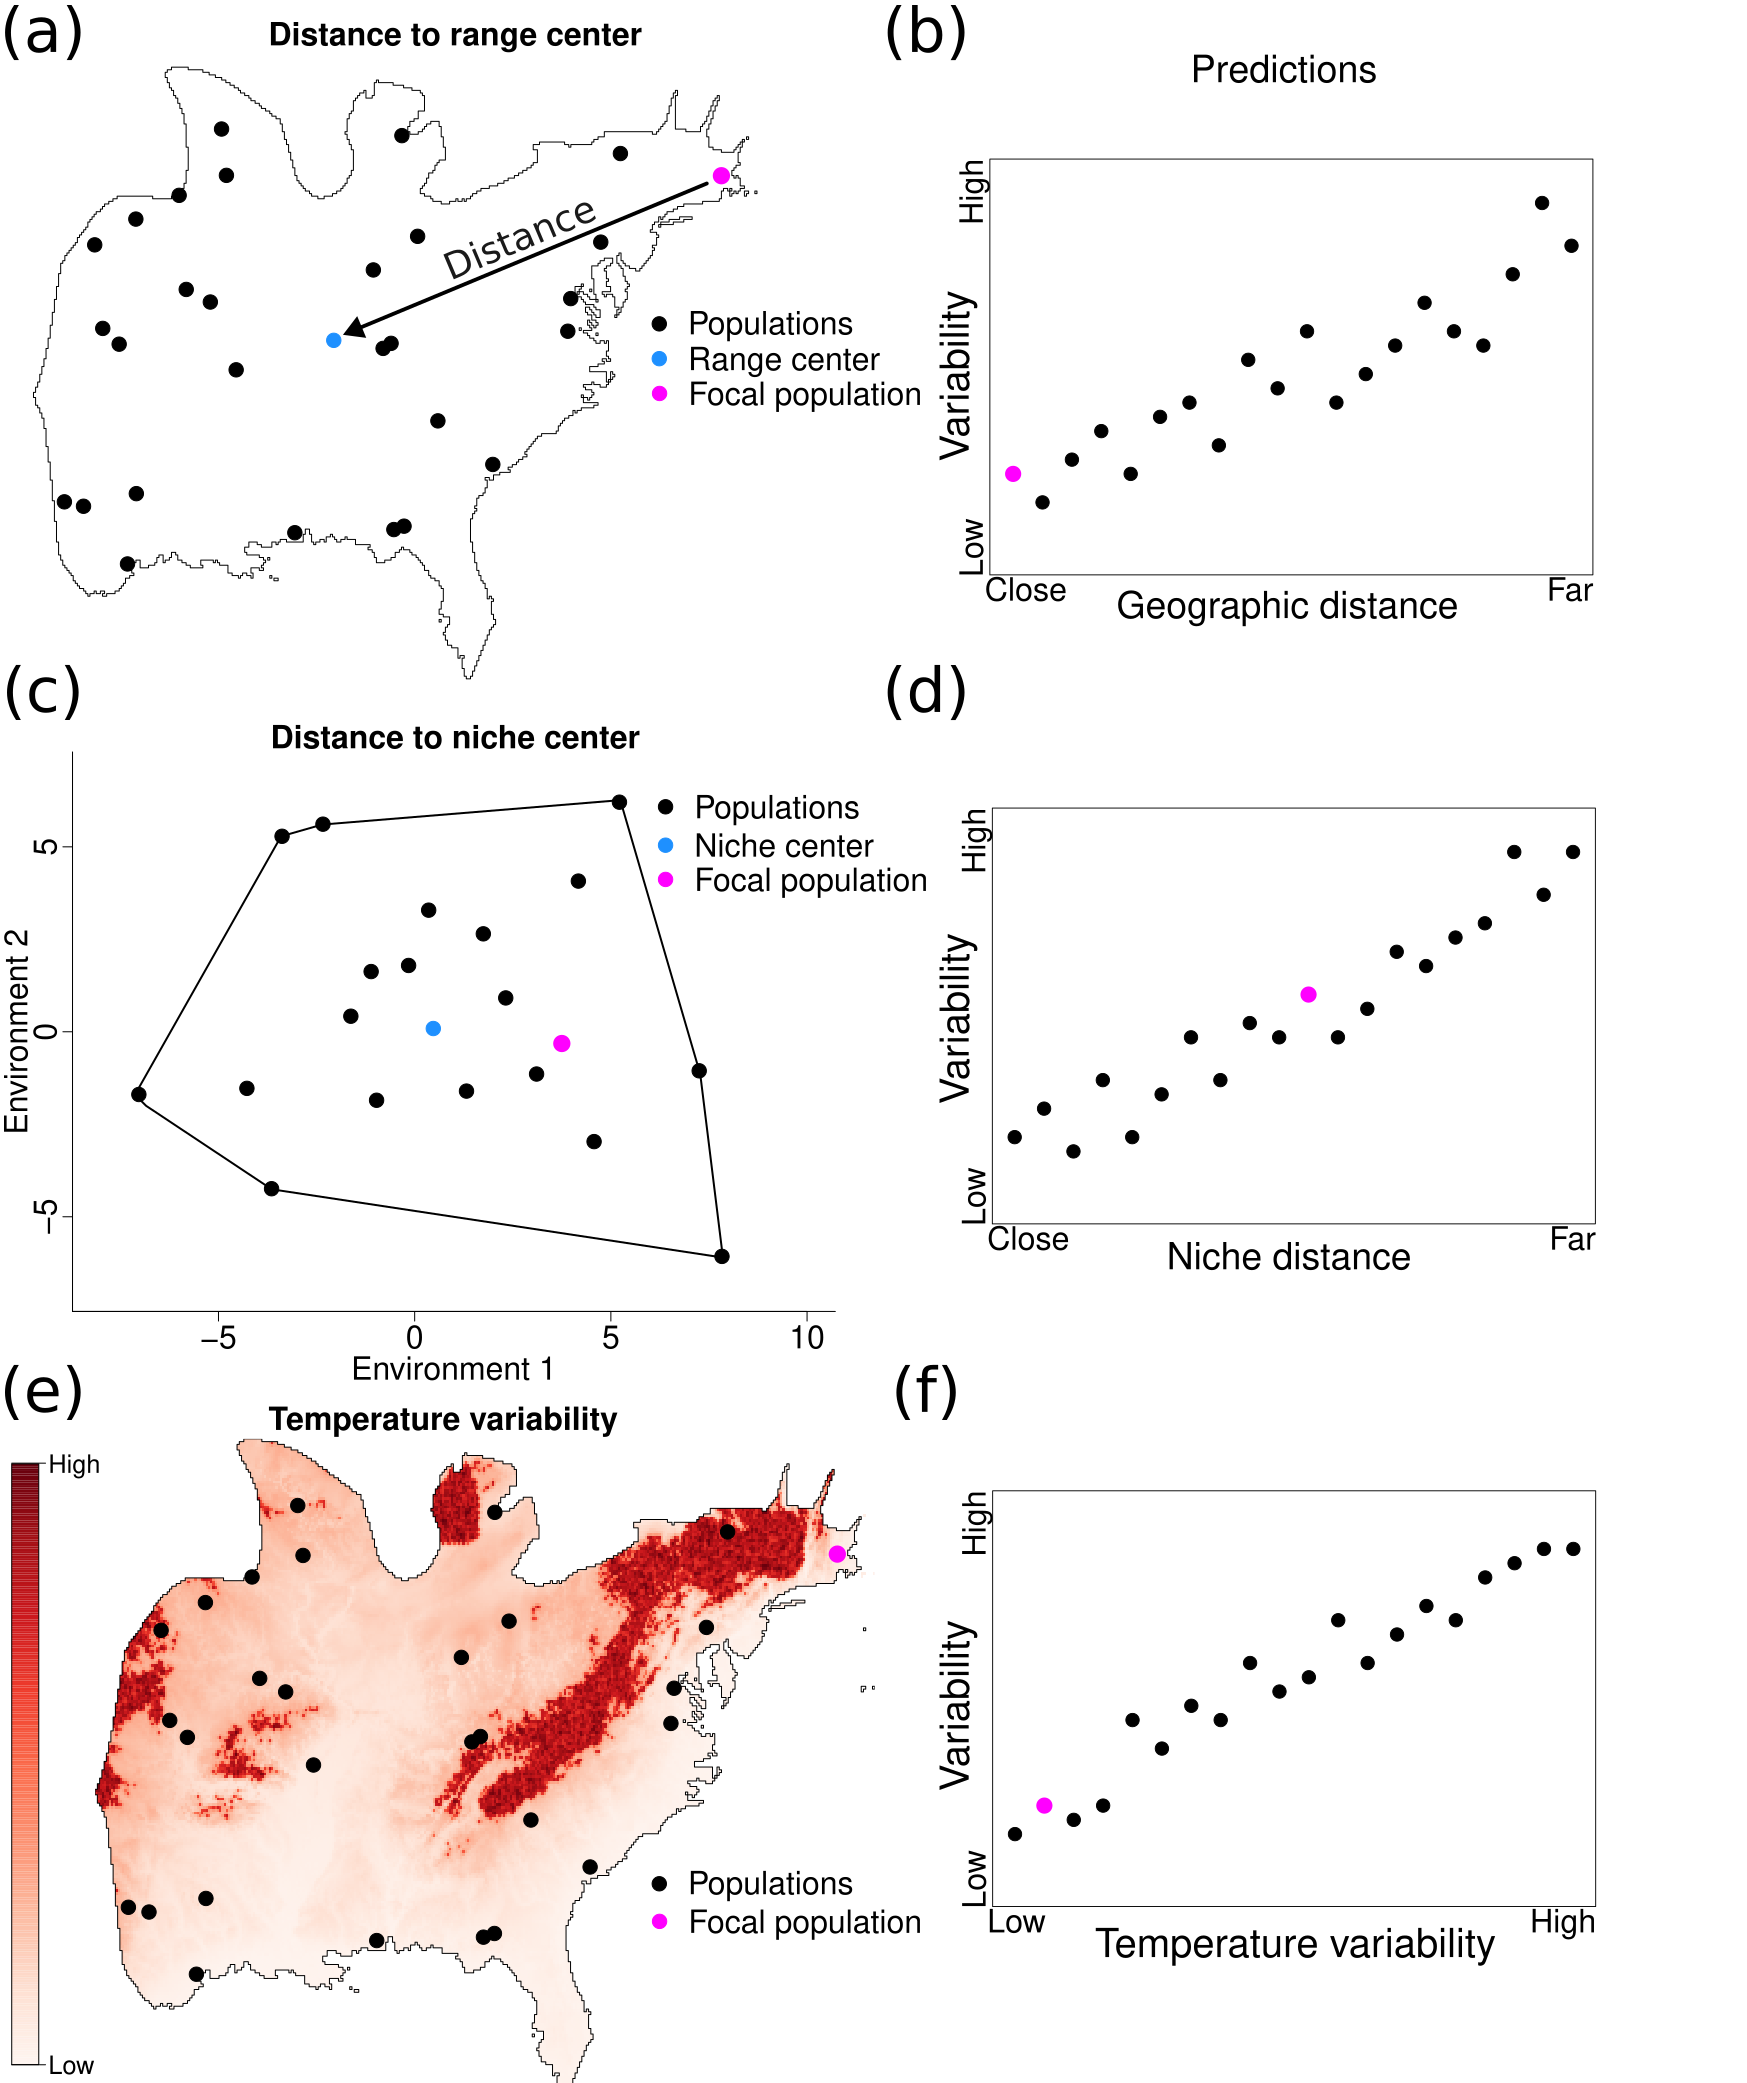
\includegraphics[width=1\textwidth]{FigRange/teste.png}}
\caption[Population variability across geographic and environmental space]{Population variability may be related to distance to geographic range center (a-b), distance to climatic niche center (c-d), or temperature variability (e-f).} 
\label{fig:concep_varrange}
\end{figure}

\begin{figure}[H]
\centering
\centerline{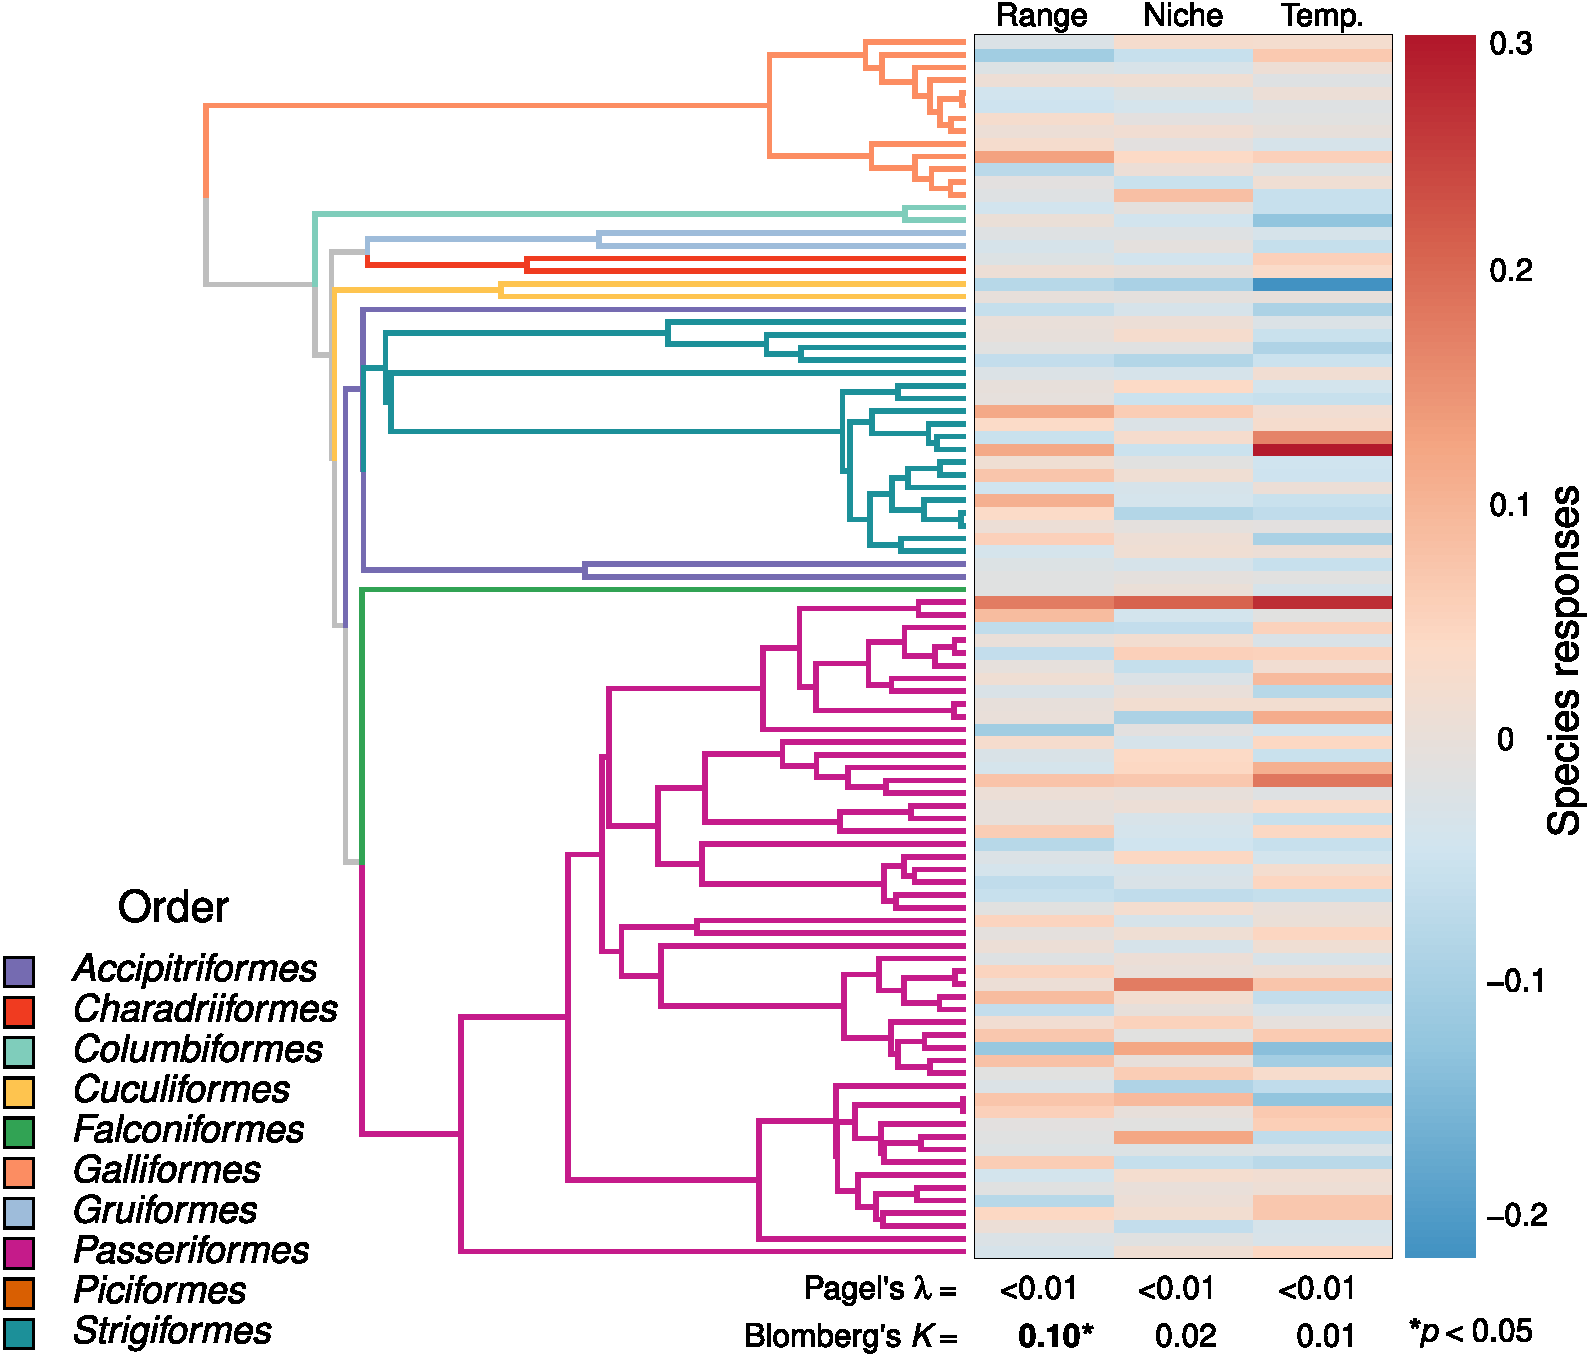
\includegraphics[width=1\textwidth]{FigRange/phyloplot}}
\caption[Phylogenetic signal on population variability]{There is no phylogenetic signal (Pagel's $\lambda$ and Blomberg's \textit{K}) in the relationship (Species responses) between climatic niche position (Niche) and temperature variability (Temp.) and population variability across species. However, there was some evidence for phylogenetic signal (Blomberg's \textit{K} = \textbf{0.10*}, p-value < 0.05) in the effects of geographic range position (Range) on population variability.} 
\label{fig:phylo}
\end{figure}

\section*{\textbf{\underline{Tables}}}

%\section*{Tables}
% latex table generated in R 4.3.2 by xtable 1.8-4 package
% Tue Jan 21 23:23:35 2025
\begin{table}[H]
\centering
  \caption[Results from linear mixed effect model]{Results from the linear mixed model showing that population variability increases near climatic niche limits (Niche) and in variable temperatures (Temp.) but not near geographic range edges (Range).}
  \vspace*{3mm}
\begin{tabular}{ccccc}
  \hline
 Predictor & Estimate & Std. Error & z value & Pr($>$|$z$|) \\ 
  \hline
  Intercept & 0.008 & 0.005 & 1.517 & 0.129 \\ 
  Niche & 0.044 & 0.013 & 3.516 & \textbf{<0.001} \\ 
  Range & 0.007 & 0.013 & 0.528 & 0.597 \\ 
  Temp. & 0.049 & 0.015 & 3.251 & \textbf{0.001} \\ 
   \hline
\end{tabular}
\label{tab:lmm_main}
\end{table}

% latex table generated in R 4.3.2 by xtable 1.8-4 package
% Wed Jan 22 08:09:11 2025
\begin{table}[H]
\centering
  \caption[Results from phylogenetic generalized least squares model]{Results from the phylogenetic generalized least squares showing the effects of body size (Body size) and dispersal ability (Dispersal) on patterns of population variability across geographic ranges (Range), climatic niches (Niche), and variable temperatures (Temp.).}
  \vspace*{3mm}
\begin{tabular}{ccccccc}
  \hline
Condition & Trait & Estimate & StdError & tvalue & pvalue & $R^2$ \\ 
  \hline
  \multirow{3}{*}[-.6ex]{\rotatebox{90}{Range}}   & Intercept & -0.025 & 0.039 & -0.637 & 0.526 & \\ 
   & Dispersal & 0.022 & 0.015 & 1.492 & 0.139 & 0.03 \\ 
   & Body size & -0.009 & 0.004 & -2.291 & \textbf{0.024} & \\\hline 
 \multirow{3}{*}[-.6ex]{\rotatebox{90}{Niche}}  & Intercept & 0.036 & 0.038 & 0.944 & 0.348 &\\ 
   & Dispersal & -0.006 & 0.014 & -0.439 & 0.661 & > 0.01\\ 
   & Body size & -0.004 & 0.004 & -0.930 & 0.355 & \\\hline 
 \multirow{3}{*}[-.6ex]{\rotatebox{90}{Temp.}}  & Intercept & 0.011 & 0.055 & 0.203 & 0.839 &\\
   & Dispersal & 0.006 & 0.021 & 0.309 & 0.758 & >0.01\\ 
   & Body size & -0.007 & 0.006 & -1.226 & 0.223& \\ 
   \hline
\end{tabular}
\label{tab:PGLS}
\end{table}

%\section*{Figures}
